\documentclass[11pt]{article}

%\usepackage{luatextra}
%\defaultfontfeatures{Ligatures=TeX}
%\usepackage{fontspec}

\usepackage{float}

\usepackage[portuges]{babel}
%\usepackage{fontspec}
\usepackage[T1]{fontenc}
%\usepackage[latin1]{inputenc}
\usepackage[utf8]{inputenc}
\usepackage[table]{xcolor}

\usepackage{microtype}

\usepackage[font=small,labelfont=bf,tableposition=top]{caption}
\usepackage[margin=1in,headheight=35pt,headsep=0.1in]{geometry}
%\usepackage[alf]{abntcite}

\usepackage{setspace}
\usepackage{amsmath}
\usepackage{amssymb}
\usepackage{amsfonts}
\usepackage{epsfig}
\usepackage[pdftex]{hyperref}
\usepackage{multirow}
\usepackage{fancyhdr}
\usepackage[nolist]{acronym}

%\usepackage{bibtex}

\listofabbreviations{Lista de Abreviaturas}
\begin{acronym}[]
	\acro{amqp}[AMQP]{{\it Advanced Message Queuing Protocol}}
	\acro{api}[API]{{\it Application Programming Interface}}
    \acro{aws}[AWS]{{\it Amazon Web Services}}
	\acro{cli}[CLI]{{\it Command Line Interface}}
	\acro{ddos}[DDoS]{{\it Distributed Denial of Service}}
	\acro{iaas}[IaaS]{{\it Infrastructure as a Service}}
    \acro{ids}[IDS]{{\it Intrusion Detection System}}
	\acro{kvm}[KVM]{{\it Kernel-based Virtual Machine}}
    \acro{ldap}[LDAP]{{\it Lightweight Directory Access Protocol}}
	\acro{nist}[NIST]{{\it National Institute of Standards and Technology}}
	\acro{paas}[PaaS]{{\it Platform as a Service}}
    \acro{rpc}[RPC]{{\it Remote Procedure Call}}
	\acro{saas}[SaaS]{{\it Software as a Service}}
	\acro{snmp}[SNMP]{{\it Simple Network Management Protocol}}
	\acro{qos}[QoS]{{\it Quality of Service}}
	\acro{sdn}[SDN]{{\it Software Defined Network}}
	\acro{vlan}[VLAN]{{\it Virtual Local Area Network}}
	\acro{vm}[VM]{{\it Virtual Machine}}
	\acro{vpn}[VPN]{{\it Virtual Private Network}}

	\acro{POV}[POF]{{\it Point of View}}

	\acro{FPS}[FPS]{{\it First-person shooter}}
	\acro{TPS}[TPS]{{\it Third-person shooter}}
	\acro{RTS}[RTS]{{\it Real-time strategy}}
	\acro{MMO}[MMO]{{\it Massively multiplayer online}}
	\acro{RPG}[RPG]{{\it Role-playing game}}
	\acro{MMORPG}[MMORPG]{{\it Massively multiplayer online role-playing game}}
	\acro{MOBA}[MOBA]{{\it Multiplayer online battle arena}}
	\acro{MMOFPS}[MMOFPS]{{\it Massively multiplayer online first-person shooter}}

	\acrodefplural{vpn}[VPNs]{{\it Virtual Private Networks}}
	\acrodefplural{vlan}[VLANs]{{\it Virtual Local Area Networks}}
	\acrodefplural{vm}[VMs]{{\it Virtual Machines}}
\end{acronym}

% Defining: \acro{acronym}[short name]{full name}
% Usaging:
% \ac{acronym}     -- writes the full name followed by the acronym in brackets; later calls will write only the acronym
% \acf{acronym}     -- writes the full name followed by the acronym in brackets
% \acs{acronym}     -- writes the short name only
% \acl{acronym}     -- writes the full name only
% Use p at the end of previous commands for plural form (e.g., \acp for the plural form of \ac)
% \acresetall        -- reset usage of all acronyms (i.e., \ac will print full name again)
% \acused                -- mark the acronym as used

%\oddsidemargin -0.7cm
%\evensidemargin -0.7cm
\topmargin -2.0cm
%\headheight 0  cm
\headsep 1.5cm
%\hoffset -1.0cm
%\footskip 40pt
%\textheight = 235mm \textwidth 185mm
\oddsidemargin 0.4cm
\evensidemargin 0.4cm
\textheight = 235mm \textwidth 165mm


\pagestyle{plain}

\usepackage{multicol}
\addtolength\columnsep{2pt}

%\newcommand{\apud}[4]{\citeauthor{#1} \mkbibparens{\citeyear{#1},\space{#2} apud \cite{#3},\space{#4}}}

\begin{document}

\pagestyle{fancy}
%\lhead{
\includegraphics[width=0.3\columnwidth]{figuras/logo_dcc.png}}
\lhead{
  
\includegraphics[scale=0.75]{figuras/logo_dcc.pdf}
}
\chead{
  \scriptsize{
    UNIVERSIDADE DO ESTADO DE SANTA CATARINA -- UDESC\\
    CENTRO DE CIÊNCIAS TECNOLÓGICAS -- CCT\\
    DEPARTAMENTO DE CIÊNCIA DA COMPUTAÇÃO -- DCC
  }
}
%\rhead{
\includegraphics[width=0.3\columnwidth]{figuras/logo_udescjlle.png}}
\rhead{
  
\includegraphics[scale=0.03]{figuras/logo_udescjlle.pdf}
}

\title{
Plano de Trabalho de Conclusão de Curso\\
Análise e caracterização de arquiteturas de microserviços empregados a jogos MMORPG voltada a otimização do uso de recursos de gerenciamento de mundos virtuais
}

\author{
Marlon Henry Schweigert -- \texttt{marlon.henry@magrathealabs.com}\\
Charles Christian Miers -- \texttt{charles.miers@udesc.br} {\it (orientador)}\\
%$<$Nome do Coorientador -- \texttt{email@coorientador} {\it (coorientador)}$>$ (se for o caso)\\
~\\
Turma 2018/1 -- Joinville/SC
}

\date{1 de Fevereiro de 2018}

\maketitle


%\singlespacing  %espaçamento simples
\onehalfspacing  %espaçamento de 1,5
%\doublespacing  %espaçamento duplo


\begin{abstract}
\noindent
  A crescente popularização de jogos massivos demanda por novas abordagens tecnológicas a fim de suprir as necessidades dos usuários com menor custo de recursos computacionais possível.
  %
  Projetar essas arquiteturas, do ponto de vista da rede, é algo pertinente e impactante para o sucesso desses jogos.
  %
  O objetivo deste trabalho é propor uma análise voltada a identificar abordagens para otimização dos recursos computacionais consumidos pelas arquiteturas identificadas.
  %
  Esse objetivo será atingido após realizar uma pesquisa referenciada, seguida de uma análise das principais arquiteturas e, preferencialmente, a execução de simulações usando uma nuvem computacional para auxiliar na identificação de gargalos de recursos. % e provendo soluções viáveis a esses problemas.
  %
  Tais otimizações dessas arquiteturas auxiliará provedores de serviços MMORPG a reduzir gastos de manutenção e melhorar a qualidade de tais serviços.

\textbf{Palavras-chave:} \textit{arquitetura de microserviços, desenvolvimento de jogos, rede de jogos, jogos massivos, otimização de recursos, nuvens computacionais}
\end{abstract}

\section{Introdução e Justificativa}
\label{sec:int}

Os avanços tecnológicos de sistemas distribuídos estão permitindo que pessoas utilizem de serviços com um grande volume de dados para aplicações sensíveis a latência. Essa situação é bem favorável a área de jogos massivos, tendo atraído pesquisadores para testar e validar novas abordagens em serviços com objetivando reduzir a carga desses serviços e reduzir o impacto a latência para o usuário final, resultando em uma melhor experiência aos jogadores da categoria de jogo tratado no presente trabalho\cite{mmo_analytic}.

O mercado de jogos massivos vem crescendo desde 2012 \cite{new_york_times}, sendo 2016 um dos mais lucrativos até então, segundo o site Statista \cite{statista_2016}. A sua projeção para 2018 é que sejam arrecadados mais de 30 bilhões de dólares americanos com esta categoria de jogos \cite{statista_2018}, um aumento de 20\% a mais sobre o ano de 2016.

\textit{Massively Multiplayer Online} ou \textit{MMO} (como são popularmente conhecidos) são os jogos de interpretação multijogador massivos, os quais surgiram de uma categoria de jogos de mesa baseados em representação de personagens. Categorizados como Role-Playing Game (RPG), um dos exemplos que pode ser citado é o jogo \textit{Dungeon and Dragons} \cite{tsr1980dungeons},  criado em 1980 e conhecido até hoje. A principal característica desse estilo de jogo é a comunicação e representação virtual de um mundo fantasia onde cada jogador pode interagir com objetos virtuais compartilhados ou tomar ações sobre outros de jogadores em tempo real, tendo como principais objetivos a resolução de problemas, o desenvolvimento do personagem e a interação entre os jogadores \cite{video_game_technologies}.

Em geral esses serviços tentem a ser sensíveis a latência e necessitam de uma demanda grande de banda, sendo por esse motivo um alvo de diversas pesquisas nas áreas de sistemas distribuidos e redes de computadores, em geral visando a minimização do impácto da latência nesses serviços\cite{stephenclarkewillson2017} e maximização de desempenho e gasto de recursos para fornecer o serviço.

Um estudo realizado \cite{system_performance} mostra um serviço clássico de MMORPG utilizando 4 servidores distintos separados por um multiplexador. Trata-se de uma arquitetura cliente-servidor a qual aguenta picos próximos a 2250 conexões simultâneas ~\ref{fig:conection_peer_hour}. Jogos de porte maior podem conter milhares de jogadores online simultaneamente. Um outro exemplo é o jogo entitulado RuneScape, a qual possui 90 mil jogadores online simultaneamente \cite{runescape_online_users}.

\begin{figure}[h]
  \caption{Plot gráfico comparando o número de conexões ao decorrer de 11 dias
  \cite{system_performance}.}
  \centering
  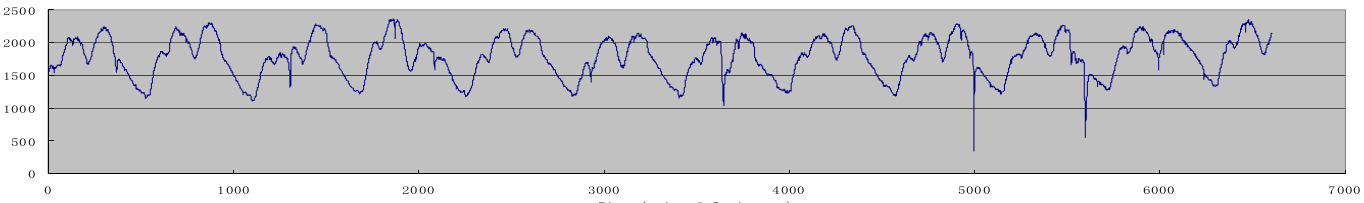
\includegraphics[width=1\textwidth]{img/connection_peer_hour.png}
  \label{fig:conection_peer_hour}
\end{figure}

Os serviços escritos atualmente, a qual podem suportar suportar milhares de jogadores, estão trabalhando como microserviços\cite{stephenclarkewillson2017}\cite{albion_online_unite}. Estes microserviços são pequenos softwares que realizam uma determinada ação de forma exemplar, uma evolução do conceito de utilidades Unix "\textit{doing one thing well}". Esses serviços pertencem a uma coleção de serviços denominada macroserviço, a qual corresponde ao serviço completo de backend da aplicação.

Os microserviços para estado de jogo são separados conforme a posição virtual do personagem do jogador. Dessa forma, regiões mais visitadas por jogadores terão maior tráfego de rede e consumo de recursos comparados a regiões pouco exploradas. Esta é uma perca grande de recurso atualmente existente nessa arquitetura \cite{cloud_fog}.

\section{Objetivos}
\label{obj}

Lorem ipsum dolor sit amet, consectetur adipisicing elit, sed do eiusmod tempor incididunt ut labore et dolore magna aliqua. Ut enim ad minim veniam, quis nostrud exercitation ullamco laboris nisi ut aliquip ex ea commodo consequat. Duis aute irure dolor in reprehenderit in voluptate velit esse cillum dolore eu fugiat nulla pariatur. Excepteur sint occaecat cupidatat non proident, sunt in culpa qui officia deserunt mollit anim id est laborum.

\section{Metodologia}
\label{met}

Para que seja possível atingir os objetivos, serão utilizados dois métodos: pesquisa referenciada, desenvolvida durante o Trabalho de Conclusão de Curso I, e pesquisa aplicada, desenvolvida durante o Trabalho de Conclusão de Curso II.


Na pequisa referenciada serão levantadas arquiteturas da literatura, buscando as mais adequadas ao escopo deste trabalho.
%
Será dividido em quatro etapas: levantamento e especificação de arquiteturas de microsserviços descritas na literatura.
%
Por fim, o levantamento e especificação de possíveis simulações para efetuar testes durante a pesquisa aplicada.

Na pesquisa aplicada, o resultado a ser obtido é a análise das arquiteturas de microsserviços definidas, visando uma análise sobre os recursos computacionais consumidos e identificação de seus gargalos.
%
Divide-se em três etapas: aplicação das arquiteturas descritas e selecionadas, realização dos testes utilizando a simulação descrita e análise dos dados coletados.

Para que os resultados sejam alcançados, são definidas as seguintes etapas:

\begin{enumerate}
  \item \textbf{Levantamento e fichamento das referências:} Pesquisa de fontes para embasamento teórico do trabalho, com base nos objetivos específicos;

  \item \textbf{Consolidação das referências:} Compreensão e seleção de artefatos literários que permitam atingir o objetivo do Trabalho de Conclusão de Curso I;

  \item \textbf{Identificação e definição de arquiteturas descritas na literatura:} Enumeração e definir das arquiteturas de microsserviços descritas na literatura, bem como os seus objetivos;

  \item \textbf{Especificação das arquiteturas selecionadas:} Especificar o funcionamento das arquiteturas selecionadas.

  \item \textbf{Identificação e definição de simulações aplicáveis ao teste:} Eleger e caracterizar a simulação a ser aplicada nos testes;

  \item \textbf{Especificação da simulação elegida:} Especificar os requisitos;

  \item \textbf{Escrita Trabalho de Conclusão de Curso I};

  \item \textbf{Desenvolvimento da simulação:} Desenvolvimento da simulação para interagir com as arquiteturas de microsserviços;

  \item \textbf{Desenvolvimento da arquitetura:} Desenvolvimento da arquitetura para executar os testes;

  \item \textbf{Aplicação das arquiteturas selecionadas na pesquisa referênciada:} Aplicação das arquiteturas descritas sobre uma nuvem computacional;

  \item \textbf{Realização dos testes utilizando a simulação elegida na pesquisa referênciada:} Execução de testes da arquitetura desenvolvida sobre a nuvem computacional;

  \item \textbf{Análise das arquiteturas testadas:} Analisar as métricas obtidas dos testes e descrever resultados, identificando possíveis gargalos nas arquiteturas;

  \item \textbf{Otimização para melhorar as métricas obtidas:} Identificar pontos de gargalo nos microsserviços identificados e propor soluções viáveis para aumentar o desempenho desses sistemas.

  \item \textbf{Escrita Trabalho de Conclusão de Curso II};
\end{enumerate}

\section{Cronograma proposto}
\label{cro}

Lorem ipsum dolor sit amet, consectetur adipisicing elit, sed do eiusmod tempor incididunt ut labore et dolore magna aliqua. Ut enim ad minim veniam, quis nostrud exercitation ullamco laboris nisi ut aliquip ex ea commodo consequat. Duis aute irure dolor in reprehenderit in voluptate velit esse cillum dolore eu fugiat nulla pariatur. Excepteur sint occaecat cupidatat non proident, sunt in culpa qui officia deserunt mollit anim id est laborum.

\section{Linha de Pesquisa}

Este trabalho será desenvolvido junto ao Grupo de Redes e Aplicações Distribuídas (GRADIS) e ao Laboratório de Processamento Paralelo e Distribuído (LabP2D). Esta pesquisa abrange as áreas de Redes de Computadores, Sistemas Distribuídos, Segurança em Redes de Computadores, Processamento Paralelo e Engenharia de Software.

\section{Forma de Acompanhamento/Orientação}

O acompanhamento será realizado principalmente através de reuniões semanais ou quinzenais, com duração máxima de 1 (uma) hora. Eventualmente as reuniões poderam ser trocadas por vídeo-conferência, troca de menssagens de correio eletrônico ou telefone. O controle das tarefas a fazer serão feitas baseadas em uma ata gerada a cada reunião. Metas semanais ou quinzenais serão atribuídas para melhor acompanhamento.


\bibliographystyle{abnt-alf}
\bibliography{tccplanoudesc}

\vskip 1.5cm

\begin{minipage} {0.49\linewidth}
  \centering
  \rule{7.2cm}{0.1mm}

  \textbf{\textit{Charles Christian Miers}}
\end{minipage}
\begin{minipage} {0.49\linewidth}
  \centering
  \rule{7.2cm}{0.1mm}

  \textbf{\textit{Marlon Henry Schweigert}}
\end{minipage}

\bigskip
\bigskip
\bigskip

\begin{minipage} {1\linewidth}
  \centering
  \rule{7.2cm}{0.1mm}

  \textbf{\textit{Rafael Rodrigues Obelheiro}}

  \textit{(Coordenador do GRADIS)}
\end{minipage}


\end{document}
